\chapter{Metaheuristic Algorithms}
\label{chpt:heuristic}
\section{Introduction}
Metaheuristics is a subdomain of the artificial intelligence domain\cite{AIModernApproach}. It evolved out of a need for more efficient search techniques with regard to hard problems. 

Metaheuristics forms part of a collective body of algorithms that use heuristics to search a particular domain's problem space for the most optimal solution adhering to certain hard and soft constraints\cite{AIModernApproach,NatureInspiredMetaHeuristic}. 

A hard constraint is defined as a certain condition an algorithm or potential solution is not allowed to violate\cite{AIModernApproach,NatureInspiredMetaHeuristic,Karen2004,Eisenblatter}. A soft constraint is allowed to be violated but there is some sort of penalty or cost involved which is imposed onto the potential solution, which lowers its desirability\cite{AIModernApproach,NatureInspiredMetaHeuristic,Karen2004,Eisenblatter}. 

An optimal solution would therefore be any solution that violates no hard constraints and violates no or a minimum number of soft constraints\cite{AIModernApproach,NatureInspiredMetaHeuristic,Karen2004,Eisenblatter}.

Some of the most famous algorithms that are classified as being part of the collective body of algorithms known as metaheuristic algorithms are:
\begin{itemize}
\item Tabu search
\item Simulated annealing
\item Genetic algorithm
\end{itemize}
The above-mentioned algorithms are not the only algorithms to form part of this subdomain, but they are the algorithms that have received the most attention in the literature and generally produce good results\cite{SweepMeta}.

The main focus of this chapter will be each of the above algorithms. Before each of the algorithms is discussed, a brief overview is given of the various characteristics that metaheuristic algorithms exhibit. 

\section{Characteristics of Metaheuristics}
NP-Complete\footnote{A discussion of NP-Complete problems is appears in section \ref{sec:NPComplete}} problems have been proven to not be solvable in polynomial time by traditional search methods such as A* search, Breath First Search and Depth-First Search\cite{AIModernApproach}. 

These traditional search algorithms are concerned with the path taken from a starting solution to a final solution. Hence, the algorithms test each and every possible solution and store any alternatives in memory since a final solution constitutes the path taken from a start node to a final node \cite{AIModernApproach}.

It is not always viable to test every possible solution in a given problem search space, especially in NP-Complete problems, since their search spaces are usually huge or infinite. This is why traditional algorithms are not able to produce optimal solutions in polynomial time\cite{AIModernApproach}.

With NP-Complete problems, the path taken from an initial possible solution to a final optimal solution is irrelevant \cite{AIModernApproach}. Only the final optimal solution is needed. Algorithms that disregard the path taken to a solution and that only care about the final solution are classified as \emph{local search} algorithms\cite{AIModernApproach}.

Local search algorithms tend to use a small amount of memory since the algorithm is only concerned with the current state and only moves to a neighbouring state when searching for a potential solution. This makes local search algorithms a good fit for optimisation problems as an optimised solution is just a solution which constitutes to the current best state found by the algorithm \cite{AIModernApproach,NonlinearGlobalTabu}. 

In its most basic form, a local search algorithm is just an algorithm that moves from one state to another. How it generates neighbouring states to move to and how and why it moves to a certain state makes the local search algorithm unique \cite{AIModernApproach,CompuIntelligenceIntro,NonlinearGlobalTabu}.

Metaheuristic algorithms are considered to be \emph{general-purpose} algorithms and can thus be applied to a wide variety of optimisation problems with only small modifications that need to made to the algorithm model\cite{MetaGraph}.

As can be gathered from the name, a metaheuristic algorithm uses some sort of heuristic. A heuristic in its most basic form is a decision rule. Algorithms use heuristics to make decisions by applying the heuristic to the data the algorithm is currently working on\cite{AIModernApproach,NatureInspiredMetaHeuristic}.

A heuristic is able to dictate what an algorithm must do for its next iteration by evaluating the current internal state of the algorithm, i.e. whether it should move to a different point in the solution space, generate new data, or select the current data as the most optimal solution\cite{AIModernApproach,NatureInspiredMetaHeuristic}.

A metaheuristic differs slightly from a normal heuristic. In general ``meta'' means \emph{beyond} or \emph{higher level}\cite{AIModernApproach,NatureInspiredMetaHeuristic}. A metaheuristic therefore refers to a heuristic that is more complex with regard to the decisions it is able to make compared with a standard heuristic\cite{AIModernApproach,NatureInspiredMetaHeuristic}.

In the literature algorithms are generally classified as being of the meta-heuristic variant when they satisfy the following criteria\cite{AIModernApproach,NatureInspiredMetaHeuristic}:
\begin{itemize}
	\item Use randomisation
	\item Use a local search
	\item Are stochastic\footnote{Exhibit behaviour that is non-deterministic.}
\end{itemize}

Metaheuristic algorithms do not search the solution space statically by testing and evaluating every possible permutation in the solution space. This is inefficient and a normal path-based algorithm can be used instead\cite{MetaAgricultural}.

Metaheuristic algorithms make use of certain strategies and heuristics (specific to the problem domain) to search the solution space intelligently through trial and error \cite{MetaAgricultural}. Intelligent searching is accomplished by combining the local search strategy along with a heuristic\cite{NatureInspiredMetaHeuristic,AIModernApproach,CompuIntelligenceIntro}. 

These algorithms iteratively move through the solution space, using a heuristic to guide the search to move to more desirable regions in the solution space where there is a high probability of obtaining high quality candidate solutions \cite{TabuMontemanniSmith,SweepMeta}.

Metaheuristic-based search methods are not guaranteed to find the most optimal solutions in the solution space; instead these methods are usually used to find near-optimal solutions. Thus most algorithmic development in the metaheuristic domain focuses on developing new techniques that will increase the probability that a good solution will be obtained in difficult combinatorial problems \cite{MetaAgricultural}.

Similarly, metaheuristics is not guaranteed to find suitable solutions or perform well in each problem domain it is applied to. The quality of the solution and performance of the metaheuristic is very much dependent upon on the expertise of the algorithm designer \cite{AutoComplexMeta}. 

The standard metaheuristic algorithm will not take advantage of specific domain knowledge as the algorithm is designed to be general purpose. Therefore for the algorithm to exploit the search domain the algorithm designer needs to embed domain-specific knowledge\cite{AutoComplexMeta,AIModernApproach}. Otherwise the algorithm will search the solution space generally and will produce relatively poor results\cite{AutoComplexMeta,AIModernApproach}.

Although heuristics plays a key role in the performance of metaheuristic algorithms, it is not the only factor that has an impact on performance and results. Algorithms also use techniques and concepts from other system paradigms like multi-agent systems\cite{Self-AdaptiveMeta}. 

In multi-agent systems, multiple agents have to communicate with each other and the system as a whole has to perform some sort of autonomous self-organisation\cite{Self-AdaptiveMeta}.

These social and self-organisation concepts enable these systems to be distributed, robust and flexible. This is why in metaheuristic algorithms that are population-based, hybrid and/or distributed, these same concepts are used to better exploit the solution space\cite{Self-AdaptiveMeta}.

In this section the characteristics of metaheuristics that set these algorithms apart from the conventional algorithms used on difficult problems was introduced. In the next section of this chapter the tabu search algorithm is discussed.

\section{Tabu Search}
\label{sec:tabusearch}
\begin{algorithm}
\caption{Basic Tabu Search Algorithm\cite{TabuRCAProblem,TabuMontemanniSmith}}
\label{alg:TS}
	\begin{algorithmic}[1]
		\STATE Initialize parameters
		\STATE $x_0 \leftarrow$ Initialize starting solution
		\WHILE{stopping criteria not met}
			\STATE $y_i \leftarrow$ Determine $x_i$ neighbourhood solutions 
			\STATE Evaluate neighbouring solutions with fitness function $f(y_i)$
			\STATE $z_i \leftarrow$Select best neighbour from $y_i$
			\IF{Move to $z_i$ is Tabu}
				\IF{$z_i$ meets Aspiration Criterion}
					\STATE $x_i \leftarrow z_i$
				\ENDIF
			\ELSE
				\STATE Add $x_i$ to Tabu List
				\STATE $x_i \leftarrow z_i$
				\IF{$x_i$ repeated $\ge$ max repeats}
					\STATE diversify()
				\ELSE
					\STATE intensify()
				\ENDIF
			\ENDIF
		\ENDWHILE
		\STATE Return $x_i$ as best found solution
	\end{algorithmic}
\end{algorithm}
\begin{figure}[p!]
	\begin{center}
	\fbox{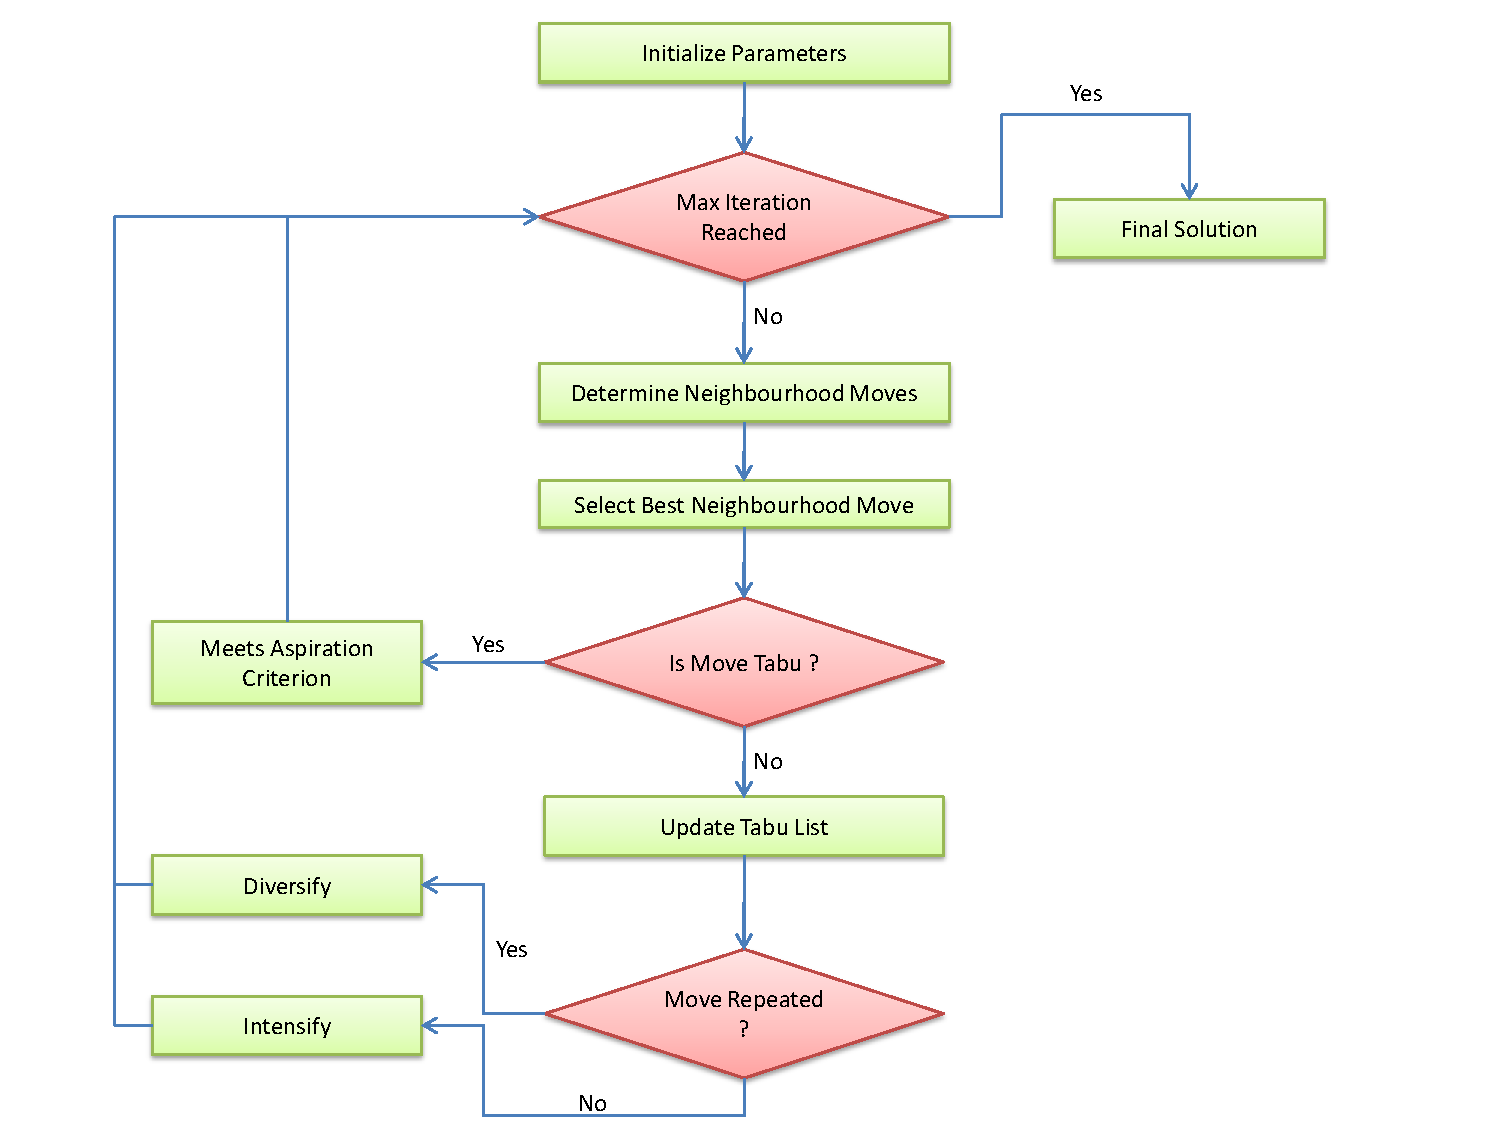
\includegraphics[width=5.0in,height=6.5in]{./pictures/TabuSearch.pdf}}
	\caption{Flow chart for tabu search algorithm}
	\label{fig:TSAlgorithmFlowChart}
	\end{center}
\end{figure}
\subsection{Introduction}
\label{sec:TSIntroduction}
Tabu search (TS) was first proposed by Glover as a new searching technique to help algorithms avoid getting trapped in local optima in combinatorial and optimisation problems \cite{TabuRCAProblem}. Since Glover introduced the algorithm in the 1980s, tabu search has been applied to a wide range of problems such as the vehicle routing problem\cite{TabuVechicleRoutingWithTimeWindows}, FAP\cite{TabuMontemanniSmith}, capacitated-lot sizing problem\cite{TabuCarryOver}, Nurse Scheduling\cite{TabuNurse} and the Resource Constrained Assignment Problem\cite{TabuRCAProblem}. 

Even though the problems mentioned differ by a large margin, the algorithm has been relatively successful in most optimisation problems it has been applied to. If one observes the results obtained in research \cite{TabuCarryOver,TabuSingleMachineScheduling,TabuVechicleRoutingWithTimeWindows,TabuBiddingStrats,TabuCrewSchedulingProblem,ReactiveTabuVHR,TabuRCAProblem,TabuCSP,TabuMontemanniSmith,tabuglobalplanning3g}, it can be deduced that tabu search has on average obtained the best results compared with previous attempts with other algorithms. 

Tabu search (TS) resembles in its most basic form the hill-climbing search algorithm\cite{TabuBiddingStrats}. The hill-climbing search algorithm starts from an initial solution and then iteratively moves from the current solution to a neighbouring solution\cite{AIModernApproach}. Each neighbour is rated based on its attractiveness as a possible optimal solution that the algorithm is being applied to\cite{AIModernApproach}. 

The hill-climbing algorithm moves to the neighbour with the highest rating without considering whether the neighbour might lead the algorithm astray, to a position where the neighbours are in fact \emph{worse} than previously encountered possible solutions\cite{AIModernApproach}. 

The TS algorithm addresses this shortcoming by introducing the concept of memory\cite{TabuBiddingStrats}. The memory of the algorithm is actually a history of previous solutions that the algorithm has moved to in its search for the problem space for a solution\cite{TabuBiddingStrats}. 

General search algorithms like hill-climbing, random-restart\footnote{Random-restart is a search algorithm where once a certain trend of repeated moves is noticed, the algorithm restarts by generating a new initial solution to start from and then continues its search process from that generated solution\cite{AIModernApproach}.} or scatter search tend to get trapped in local optima \cite{AIModernApproach}. The local optima might be a very attractive solution and thus general search algorithms will not move to better solutions since, according to the algorithm's built-in strategy, it has found the best solution. 

In actual fact the solution that was found is the best solution in the \emph{local} search space, but not in the \emph{global} search space\cite{CompuIntelligenceIntro,AIModernApproach}. Therefore an important characteristic of algorithms being applied to optimisation problems is breaking out of local optima\cite{CompuIntelligenceIntro,AIModernApproach}.

In an attempt to better understand the algorithm, the flow of the TS algorithm is set out below.
\subsection{Flow of the algorithm}
The general flow of the TS algorithm is described using algorithm~\ref{alg:TS} as a reference point.

Before the algorithm can actually start searching, it first needs to initialise various parameters. These parameters include, but are not limited to, the tabu list size, the aspiration criterion and the starting solution. The initialisation can be observed to occur from lines 1 - 2.

Once all the various parameters that are needed by the algorithm have been initialised, the algorithm is ready to enter the actual search phase, which ranges from lines 3 -- 21. 

The search phase starts off by first generating possible solutions that neighbour the current solution $x_i$ as can be observed in line 4. Generating neighbouring solutions are a critical process in the TS algorithm as tehy are the means by which the algorithm is able to move from one possible solution to the next in the search space. Neighbourhood search will be discussed in detail in section~\ref{sec:TScharacteristics}.

After all the solutions that neighbour the current possible solution have been generated, the algorithm needs to decide which of the possible neighbours is the most lucrative. The algorithm therefore determines the fitness of each neighbour $y_i$ by applying a fitness function $f(y_i)$. 

Once all the neighbours have been evaluated, the algorithm selects the best neighbour that not only has the best fitness out of all the generated neighbours, but also has a better fitness than the current solution held by the algorithm. The best neighbour selection can be seen to occur in line 6.

The algorithm has now determined a possible neighbour $z_i$ to move towards. Before moving on to the next iteration, it first needs to perform a series of checks that will aid it in the search process.

The first check that needs to be performed is whether the neighbour $z_i$ is in the tabu list and this occurs in line 7. A solution is only in the tabu list if the algorithm has in a previous iteration had the particular solution as its current solution. Tabu lists will be discussed in section~\ref{sec:TScharacteristics}.

If the neighbour $z_i$ is in the tabu list, then another check is performed where the aspiration criterion is calculated as can be seen in lines 8 -- 10. The aspiration criterion determines whether the algorithm can make neighbour $z_i$ its current solution once more even though it is tabu. 

If the aspiration criterion has been met, the algorithm makes neighbour $z_i$ its current solution $x_i$. More will be discussed on the aspiration criteria in section~\ref{sec:TScharacteristics}.

When a solution is not in the tabu list, it could possibly mean that it is the first time the algorithm has encountered the solution, or the solution has been previously encountered, but has been removed from the tabu list. A solution can be removed from the tabu list once it has been tabu for a certain number of iterations. More will be said on how the tabu list is updated in the next section.

In the algorithm, if a neighbour $z_i$ is found not to be in the tabu list, the algorithm then adds the currently held solution $x_i$ to the tabu list. The current solution is added to prohibit future movements to the same solution in an attempt to avoid cycling of solutions. After $x_i$ has been added to the tabu list, the algorithm makes $z_i$ the current solution $x_i$. This process can be observed from lines 12 -- 14.

Before the algorithm continues to the next iteration, it performs one last final check. The purpose of this check is to determine whether the algorithm is repeating solutions. As can be observed from lines 15 -- 19, the algorithm calculates whether the new selected solution has been repeated for a certain number of iterations. 

If the solution has indeed been repeated for a predetermined number of iterations, the algorithm activates its diversification strategy or intensifies its search. These two strategies are discussed later.

\subsection{Important Tabu Search Characteristics}
\label{sec:TScharacteristics}
Various characteristics are important to the TS algorithm. The first characteristic is exactly how the TS algorithm iteratively improves upon the initial start solution.

\subsubsection{Initial Solution Generation}
The core feature of the TS algorithm is to sequentially improve an initial solution \cite{TSHazardous}. An initial possible solution is a point in the problem space where the TS algorithm will \emph{start} exploring in search of a more optimal solution \cite{AIModernApproach,TSHazardous}.

An important consideration one has to make is how initial solutions are generated for the TS algorithm to start on\cite{AIModernApproach,TSHazardous}.

Random initial solutions might seem to be a good starting point, but by introducing randomisation it becomes hard to control the quality of the end solution\cite{TSHazardous}. Hence the generation of starting solutions must be controlled to limit the infeasibility of potential solutions \cite{TSHazardous}. 

Control of the randomly generation solutions can be achieved by simply constraining the random solution generator to only generate initial starting points in a bounded subset of the entire search space. For example: instead of letting the random initial starting point be any number between positive infinity and negative infinity, the random number generator is constrained to only generate numbers between 5 and -5.

\subsubsection{Neighbourhood Search}
TS uses a neighbourhood local search process to explore the solution space. There is no set process of how neighbourhood candidate solutions are selected. Depending on the problem to which the TS is applied, different neighbourhood solution selection strategies are needed. The overall quality of the solution produced by TS is also dependent on the neighbourhood search strategy used \cite{TSHazardous}. 

As can be observed from the TS flow chart in figure \ref{fig:TSAlgorithmFlowChart} the neighbourhood search phase is the first operation performed after the algorithm has been initialised, which is to say the algorithm has generated an initial starting solution from which the exploration process can start.

The neighbourhood search phase is the primary means for the TS algorithm to search the solution space for an optimal solution. It is within this phase that new possible solutions must be presented for the TS heuristic to allow the algorithm to decide to which solution it must move next.

The new possible solutions that are generated are called neighbouring solutions; hence the TS algorithm always moves to a neighbouring solution. When the TS algorithm moves to a neighbouring solution, the current solution is replaced by the neighbouring solution. Therefore, in the next iteration, neighbours for the new solution need to be generated.

Generation of new neighbours can range from a simple increment option to a complex operation that incorporates additional intelligence by means of a more heuristic approach to generate new neighbours.

The TS algorithm is not limited to just one neighbourhood search strategy. In the paper by Gopalakrishnan et al.\cite{TabuCarryOver} five neighbourhood move strategies are developed and are used interchangeably; in some cases a strategy is used three times in a row due to stagnation in the search space. 

Stagnation occurs when the algorithm does not move to a better solution; instead it opts to stay on the current solution, as no neighbouring solution is better than the current one. However, to combat this stagnation, the authors opted to use all the move strategies 15 per cent of the time, and the last four move strategies for 85 per cent of the time when generating neighbourhood solutions.

Other neighbourhood strategies developed is that by N. A. Wassan \cite{ReactiveTabuVHR}. In that author's paper a neighbourhood selection strategy is used that exchanges route nodes from initial vehicle routes for the vehicle routing problem. This route exchange enables the TS algorithm to search much more broadly due to the constant supply of different solutions. 

Since initial solutions are constantly modified, it enables the TS procedure to be a very fined-grained process, because often a small change in a potential solution can have a big impact on the overall proposed solution by the TS algorithm.

In the research done by Zhang et. al.\cite{TSHazardous} an interesting neighbourhood selection scheme called \emph{dynamic penalty} is developed. When the algorithm moves onto an infeasible solution a penalty is imposed. By dynamically changing the penalty that is imposed the ``feasibility'' of solutions produced is influenced. 

Therefore, if and when the algorithm continually produces infeasible solutions, the penalty imposed is increased to guide the algorithm to produce more feasible solutions. Finally, when the algorithm gets trapped at local optima, the penalty is reduced, which allows the algorithm to consider moving onto infeasible solutions thus escaping local optima.

Considering all the research done to develop new neighbourhood selection strategies that improve TS to search the solution space more efficiently and produce better, faster solutions, TS still has some drawbacks, especially with problems that have very large solution spaces \cite{EvoParallelTabu}.

TS is an iterative algorithm, executing a set of operations sequentially until a stopping criterion is met as can be seen in the flow diagram. At each iteration the algorithm has to determine feasibility of the immediate neighbourhood candidate solutions \cite{EvoParallelTabu,TabuVechicleRoutingWithTimeWindows}. 

Therefore each candidate must be evaluated by some function, which may be a costly operation in terms of computational cycles as well as in terms of time. This constant evaluation can drastically reduce the overall performance of the algorithm, since it is spending more time calculating feasibility than actually searching the solution space \cite{EvoParallelTabu,TabuVechicleRoutingWithTimeWindows}.

\subsubsection{Memory Structures of Tabu Search}
The hill-climbing and random-restart algorithms are able to break out of local minima, but there is nothing stopping these algorithms from avoiding the local optima with their second or n-pass in the search space. TS addresses the shortcoming of these algorithms by incorporating an important concept: the notion of memory.

In its most basic form TS keeps a local memory of all its recent best moves, and puts them into a \emph{tabu list} that has a predefined size. In the literature the Tabu list is also referred to as the \emph{tabu tenure} \cite{TSHazardous,TabuCarryOver,ReactiveTabuVHR,TabuParameterization}. The algorithm is not allowed to move to any solution that is in the tabu list unless a solution that is \emph{tabu} is better than any current moves available in the immediate search neighbourhood \cite{TSHazardous,TabuCarryOver,ReactiveTabuVHR,TabuParameterization}. The process of overriding a solution's tabu status in the tabu tenure is called the \emph{aspiration criterion} \cite{TSHazardous,TabuCarryOver,ReactiveTabuVHR,TabuParameterization}. With the use of the tabu tenure and the aspiration criterion, the algorithm is able to avoid cycling, local optima as well as searching in a too narrow region \cite{TabuSingleMachineScheduling,CircuitTabu}.

Research done by Ashish Sureka and Peter R. Wurman makes an important distinction with regard to the memory scheme that is used in the TS algorithm. Two memory schemes are discussed: \emph{explicit memory} and \emph{attribute-based memory} \cite{TabuBiddingStrats,TabuFormGames}. Of the two memory schemes the explicit memory scheme is the most used in the literature \cite{TabuVechicleRoutingWithTimeWindows}.

With explicit memory the algorithm stores a complete solution in the tabu tenure; hence the algorithm is prohibited from moving to that position in the solution for as long as the solution is in the Tabu tenure\cite{TabuBiddingStrats,TabuFormGames}. With attribute-based memory the algorithm stores the \emph{operation} used to move from the previous solution to the current solution\cite{TabuBiddingStrats,TabuFormGames}. Therefore with attribute-based memory the tabu tenure intended function is changed from prohibiting certain solutions already encountered to rather prohibiting making changes to the current solution that would lead to solutions already present in the tabu tenure \cite{TabuBiddingStrats,TabuFormGames}.

In research conducted by D. M. Jaeggi, G.T. Parks, T. Kipouros and P. J. Clarkson \cite{MultiObjTabu}, the authors add two additional memory structures called \emph{medium term memory} (MTM) and \emph{long term memory} (LTM) besides the standard \emph{short term memory} (STM), typically referred to as the tabu List \cite{MultiObjTabu}. Each additional structure remembers a different set of solutions for use by the diversification and intensification phases in the algorithm.

STM is similar to the traditional tabu list: to store the most recent solutions produced by the algorithm. MTM is designed to remember optimal or near-optimal solutions. These solutions are therefore used later in the intensification phase. Finally, the LTM structure stores all the regions that the algorithm has already explored and is thus used in the diversification phase of the algorithm \cite{MultiObjTabu}.

\subsubsection{Search Phases}
As TS searches through the solution space, it goes through two cycles of search phases called \emph{diversification} and \emph{intensification} \cite{TabuParameterization,TabuCrewSchedulingProblem,NonlinearGlobalTabu,SelfControllingReactiveTabu}.

The diversification phase in the TS algorithm is the phase where the algorithm is directed to areas in the solution space that has not yet been explored. The algorithm usually applies diversification as mechanisms monitoring the memory; note that solutions being produced are being repeated \cite{ReactiveTabuVHR,SelfControllingReactiveTabu}. 

Fescioglu-Unver and Kokar \cite{SelfControllingReactiveTabu} researched a strategy is presented that consists of two components namely the \emph{observer} and the \emph{diversifier}. The goal of the observer is to continually monitor the best solution obtained by the algorithm as to whether it violates the \emph{stagnation period}. The stagnation period is defined as the number of iterations where the current best obtained solution has not changed \cite{SelfControllingReactiveTabu}. 

As soon as the algorithm exceeds the stagnation period the observer component activates and transfers the necessary information needed by the diversifier component. The diversifier component dynamically changes the size of the tabu tenure based on the information the observer gathered. The diversifier mainly targets older moves to diversify, but for short bursts of time it decreases the tabu list size to a very small value in an attempt to combine new and old moves \cite{SelfControllingReactiveTabu}.

The specific mechanism used to define a new position where the algorithm can continue to search, should ideally select areas in the solution space that have not been explored yet. Therefore, the diversification phase typically makes extensive use of the knowledge present in the long-term memory structures as an indication of what areas of the solution space have been previously explored and which areas have not \cite{TabuParameterization,TabuCrewSchedulingProblem,NonlinearGlobalTabu,SelfControllingReactiveTabu}.

Intensification is usually the first phase of the TS algorithm, since it is responsible for building up a history in memory on which the diversification phase can act. Fescioglu-Unver and Kokar also present an intensification strategy based on control theory in their research \cite{SelfControllingReactiveTabu}. The authors identify repetition length as a critical value for their intensification strategy to be based upon. The repetition length is a control measure that defines how many times a solution may be repeated.

In the following section, an overview will be presented of literature that used the TS algorithm on the FAP.
\subsection{Tabu Search on the FAP}
As discussed, the TS algorithm is an optimisation algorithm and has been applied to a wide variety of optimisation problems (see page \pageref{sec:TSIntroduction}). In the literature the TS algorithm has also achieved relatively good results.

In a study conducted by Robert Montemanni and Derek Smith \cite{TabuMontemanniSmith} the TS algorithm is used on the FS-FAP. Since the TS algorithm is generic, the authors had to make some alterations to the algorithm to suit their needs as well as to make the algorithm more efficient in exploring in the FAP solution space.

The TS algorithm used by the authors is the multistart TS algorithm, which randomly starts on different initial solutions \cite{TabuMontemanniSmith}.

The authors developed a technique called heuristic manipulation technique (HMT). HMT first monitors an underlying heuristic being used on the problem by the algorithm\cite{TabuMontemanniSmith}. It then identifies certain characteristics that good solutions exhibit. In the FAP, it is transmitters that are assigned different frequencies which results in an overall lower interference value\cite{TabuMontemanniSmith}.

The HMT then uses the identified characteristics to add \emph{additional} constraints to the problem\cite{TabuMontemanniSmith}. By adding constraints, the search space is reduced, which therefore makes it easier for the algorithm to find an optimal solution, as there are fewer solutions to consider. However, by reducing the search space, other near-optimal solutions which might be far better are excluded\cite{TabuMontemanniSmith}. It is for this reason that the authors opted not to add the constraints permanently, instead the constraints are replaced by other constraints\cite{TabuMontemanniSmith}.

The authors applied their TS algorithm together with HMT to the COST 259 family of benchmarks, specifically the Siemens1, Siemens2, Siemens3 and Siemens4 problems.
\begin{table}
\centering
	\begin{tabular}{| c | c | c |}
		\hline
		Problem instance & TS with HMT & Best COST 259 \\ \hline
		Siemens1 & 2.7692 & 2.200 \\ \hline
		Siemens2 & 14.9360 & 14.280 \\ \hline
		Siemens3 & 6.6496 & 5.19 \\ \hline
		Siemens4 & 110.9725 & 81.89 \\ \hline
	\end{tabular}
\caption{Results of applying TS with HMT on COST 259}
\end{table}
As can be observed from the results obtained by the authors, the TS algorithm with HMT produces results that rank very favourably against other algorithms also applied to the COST 259.

When critically evaluating the TS algorithm with regard to applying it to the FAP, the following disadvantages can be identified:
\paragraph{Search based on a single solution}
--- The TS algorithm at any moment in time only searches in the vicinity of \emph{one} current solution for possible neighbours that might be the current solution for the next iteration. FAPs typically have huge search spaces due to their NP-Hard nature. Therefore, only searching for possible lucrative neighbours from only potential solutions seems to be terribly inefficient. A better strategy would be to use the notion of population-based algorithms and have multiple solutions from which lucrative neighbours are searched.
\paragraph{Neighbourhood generation}
--- The TS algorithm defines no set process for generating a neighbouring solution given a starting solution. Generating neighbours from a solution is a critical process in the TS algorithm, for it is the only means by which the algorithm considers other solutions, i.e. it is the mechanism by which the algorithm searches. Generating a new neighbour can be as simple as changing only one value from the current solution or it can be very complex and incorporate other algorithms together with mathematics formulae. Regardless of the complexity of the neighbour generation that is used, care must be taken to ensure that the algorithm is able to produce a wide diversity of neighbours and is also able to intensify on the most optimal solution.
\paragraph{Tabu lifetime}
--- The TS algorithm only operates on a single solution at a time and at most only considers one potential neighbour as its next possible current solution. Therefore a difficult choice needs to be made as to how long a solution stays tabu. In the FAP a solution might be entered into the tabu list early in the search process of the algorithm. A large majority of the neighbours of this solution are vastly superior solutions compared with any of the current solutions produced by the algorithm. Due to the solution with these neighbours being in the tabu list, these neighbours will not be reconsidered until much later when the solution is removed from the list. The only other option is if the aspiration criterion is met, which is another parameter which needs to be fine-tuned. A high aspiration criterion and the algorithm might be too eager to select just any solution even though it is Tabu. A low aspiration criterion and the algorithm will be too strict in selecting a tabu solution.

In the next section the simulated annealing algorithm is discussed.
\section{Simulated Annealing}
\label{sec:simulatedannealing}
\begin{algorithm}
\caption{Basic Simulated Annealing Algorithm\cite{VeryFastSAImageEnchancement,ChaosSA}}
\label{alg:SA}
	\begin{algorithmic}[1]
		\STATE Initialize parameters
		\STATE Set starting temperature $T(0)$
		\STATE $x_0 \leftarrow$ Generate initial starting solution
		\WHILE{Stopping criteria not met}
			\STATE $y_i \leftarrow$ Generate neighbouring solutions to $x_i$
			\STATE Evaluate $y_i$ neighbours with fitness function $f(y_i)$
			\STATE Calculate probability $p_i$ of $y_i$ neighbours with equation~\ref{eq:saprobability}
			\STATE $x_i \leftarrow$ Select $y_i$ neighbour based on probability $p_i$
			\STATE Reduce temperature $T(i)$ based on cooling schedule
		\ENDWHILE
		\STATE Return best solution $x_i$
	\end{algorithmic}
\end{algorithm}
\begin{figure}[htbp!]
	\begin{center}
	\fbox{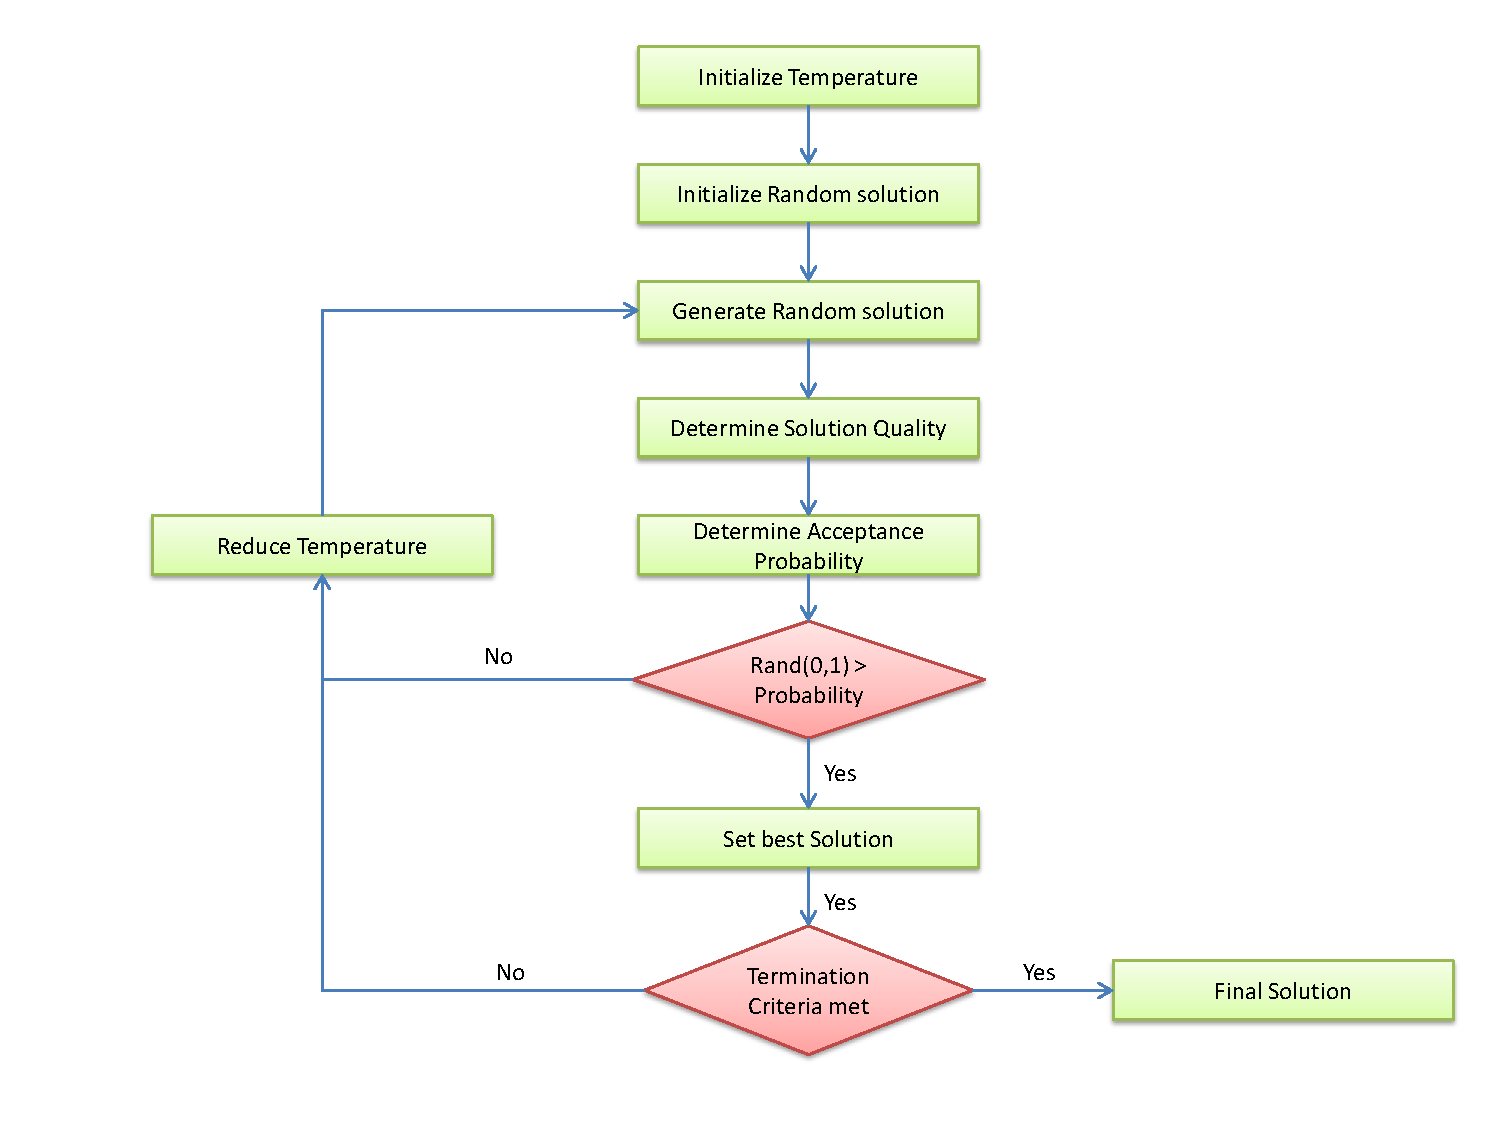
\includegraphics[width=5.0in,height=5.5in]{./pictures/SimulatedAnnealing.pdf}}
	\caption{Flow chart for simulated annealing algorithm}
	\label{fig:SimulatedAnnealingFlowChart}
	\end{center}
\end{figure}
\subsection{Introduction}
\label{sec:SAIntroduction}
Simulated annealing (SA) is a heuristic search technique proposed in the 1980s by Kirkpatrick to solve combinatorial optimisation problems. The technique is based on a natural process which is known in metallurgy as annealing \cite{CurveFittingSA,SASingleMultiObj,TempCyclingSA,ChaosSA}. Kirkpatrick was the first to use SA to solve optimisations problems but the basic algorithm structure was defined by Metropolis et al. in 1953 \cite{CurveFittingSA,VeryFastSAImageEnchancement}.

Annealing is the natural process of crystallisation when a solid is heated to a high temperature and then systematically cooled to a lower temperature to reach a crystallised form \cite{CurveFittingSA,NewSAs,MobileRobotSA,ConstantTempSA}. This crystallised form of the solid is known to be the global minimum of the solid's internal energy state. 

When the solid is rapidly cooled from a high temperature, the molecules have no time to reach a thermodynamic equilibrium stage \cite{CurveFittingSA,NewSAs,MobileRobotSA,ConstantTempSA}. Therefore the molecules of the solid have high energy and the resultant structure has no real crystalline form; thus the solid energy is at a local minimum\cite{CurveFittingSA,NewSAs,MobileRobotSA}. When the solid is slowly cooled in a controlled manner, the molecules are able to reach a thermal equilibrium at each temperature \cite{ChaosSA,CurveFittingSA,NewSAs,MobileRobotSA,ConstantTempSA}.

In the algorithm the energy state is the \emph{cost function} that needs to be minimised, and the molecules are the \emph{variables}, which represent the solutions, and thus their state needs to be optimised to reach the desired energy state.

The following equation is the standard probability function that is used to determine when an uphill move is performed by the algorithm. This function is known in the literature as the \emph{metropolis criterion}. 
\begin{equation}
\label{eq:saprobability}
	M_{AC} =
	\begin{cases}
	1, &\text{if $f(y) \leq f(x)$}\\
	exp(-\frac{\Delta E}{T_k}), &\text{otherwise}\\
	\end{cases}
\end{equation}
The function $f$ is the objective function or a function that determines the state of a given position in solution space\cite{EcoEquilSA}. The parameter $T_k$ is the temperature of the algorithm at iteration $k$ \cite{EcoEquilSA}. Finally, $\Delta E$ is the change in ``energy'' between two solutions $x$ and $y$ \cite{EcoEquilSA}.

The main purpose of the SA algorithm (like most optimisation algorithms) is to minimise or maximise the cost function \cite{SASingleMultiObj}. This cost function typically evaluates a solution desirability compared with other solutions in the immediate \emph{neighbourhood} of the algorithm's current position \cite{TheoPraticalSA}. 

The immediate neighbourhood of solutions is generated based on some heuristic implemented by the algorithm designer\cite{AIModernApproach}. This heuristic, as with the TS algorithm, can be simple or complex. The neighbourhood generated is the first step right after the starting solution has been generated by the algorithm, as can be observed from figure \ref{fig:SimulatedAnnealingFlowChart}.

Typically a neighbouring solution is only selected as the new best state if its desirability ranks higher than the current solution. When the algorithm moves to a better solution from the previous solution, the move is typically referred in the literature as a \emph{downhill} move \cite{CurveFittingSA}.

The best state is not always selected; in some cases the algorithm is also able to move to solutions that are worse than the current solution. A worse solution is only selected based on some probability which is controlled by the \emph{annealing temperature} of the algorithm \cite{TheoPraticalSA}. 

At a high annealing temperature the probability that the algorithm will select a bad solution is very good. As the annealing temperature decreases so does the probability that a bad solution will be selected \cite{CurveFittingSA}. When the algorithm moves to a worse solution, the move is typically referred to in the literature as an \emph{uphill} move \cite{CurveFittingSA}. Uphill moves allow the algorithm to break out of local minima and can lead the algorithm down a different path, which may ultimately result in obtaining the global optimum \cite{SASingleMultiObj}. 

The SA algorithm is also very popular due to its basic structure being generic\cite{VariousCoolingSA}. As with the TS algorithm, the standard SA algorithm does not define a set neighbourhood generation mechanism; instead it is up to the algorithm designer to implement a suitable generation mechanism that will allow the algorithm to adequately explore the problem space\cite{VariousCoolingSA}. 

Applying the algorithm to other problems requires slight changes. These changes usually need to be applied to the \emph{neighbourhood selection} scheme and the \emph{cooling schedule}\cite{VariousCoolingSA,DormRoomSA}. Both of these concepts will be discussed below.

\subsection{Flow of the Algorithm}
In an attempt to better understand how the SA algorithm operates, a general discussion on the flow of the algorithm will now be given using algorithm~\ref{alg:SA} as a reference point.

From lines 1 -- 3, the SA algorithm is initialised. The most important step here is setting the starting temperature for the annealing process to start. As mentioned in the introduction, the temperature of the annealing process plays a critical role in the potential solution selection process.

After the algorithm has been initialised the search phase of the algorithm starts which ranges from lines 4 -- 10. Like the TS algorithm, the SA algorithm starts the search phase by generating a number of neighbours to the current solution held by the algorithm as can be observed in line 5.

Before selecting a neighbour the algorithm first needs to evaluate the generated neighbours. It evaluates each neighbour by applying a fitness function $f(y_i)$ in order to determine its fitness.
Once the fitness of all the generated neighbours has been determined, the algorithm uses equation~\ref{eq:saprobability} to calculate the probability of selecting a particular neighbour for all the generated neighbours as well. The probability calculation can be observed to occur in line 7. The algorithm then selects the neighbour with the highest probability to be the current solution, as observed in line 9. 

Before the algorithm advances to the next iteration the temperature needs to be lowered. The temperature is a critical variable as it has a role in the probability equation and therefore can affect solution selection. The temperature is not simply lowered with a subtraction operation, but rather according to a particular cooling schedule. In the algorithm the process of lowering the temperature occurs in line 10.

The characteristics that were briefly mentioned in the introduction section will now be discussed in more detail.
\subsection{Important Simulated Annealing Characteristics}
There are four characteristics of the SA algorithm that make the algorithm unique. One of the most important is the cooling schedule. 

%\subsubsection{Markov Chain}
%The SA Algorithm is typically modelled by using Markov chains due to each Markov chain represents a set of trials that the algorithm has executed at the same temperature. 

%A Markov chain\footnote{Also known as Markov process} defines a chain of states or processes that satisfy the \emph{Markov assumption}. Which is defined as, that any state only depends on a set amount of previous states that have been encountered previously\cite{AIModernApproach}.
%%
%It has been proven with the use of Markov Chain theory that SA will find the global minimum in the solution space \cite{ClusterSA}. This proof is only valid when the following properties for the underlying Markov chain hold \cite{VeryFastSAImageEnchancement}:
%\begin{itemize}
%\item It must be irreducible
%\item It mustn't be periodic
%\item The detailed balance condition must hold
%\end{itemize}
%According to the proof presented in \emph{Image enhancement using very fast simulated reannealing}\cite{ClusterSA}, if the SA algorithm designer can uphold the above properties, the algorithm is able to find the global optimum. Even though the algorithm will eventually find the global optimum, the algorithm is known to take a very long time to do so.
\subsubsection{Cooling Schedule}
The cooling schedule/annealing Schedule is the most defining characteristic of the SA algorithm. It is the procedure where the natural annealing process is mimicked. The temperature of the SA algorithm is a control parameter that defines how much the algorithm moves around in the solution space.

As can be observed from figure \ref{fig:SimulatedAnnealingFlowChart}, after each iteration, whether the algorithm has selected a new best solution or not, the temperature is reduced by a certain amount. This amount is determined by the cooling schedule.

In general, when the SA algorithm temperature has a very high value most solutions that are produced from the neighbourhood are accepted \cite{ClusterSA}. Thus the algorithm moves freely in the solution space with little constraint. As the temperature decreases, the probability that the algorithm will select a bad or just any solution decreases. When the temperature is very low, the SA algorithm is similar to a greedy algorithm in the sense that it only accepts downhill movements\cite{ClusterSA}.

In the literature there are three annealing schedules in common use, namely \emph{the logarithmic schedule}, the \emph{geometric schedule} and the \emph{Cauchy schedule}\cite{VeryFastSAImageEnchancement,SASingleMultiObj}. 

The standard and most commonly used schedule is known as the logarithmic schedule and is based on Boltzmann annealing \cite{VeryFastSAImageEnchancement}. The main disadvantage of this schedule is that is slow due to its logarithmic nature \cite{VeryFastSAImageEnchancement}. It also requires moves to be generated from a Gaussian distribution for it to be able to reach the global minimum\cite{SASingleMultiObj}. The logarithmic annealing function has the following form:
\begin{equation}
\label{eq:logcooling}
	T_k = \frac{T_0}{ln(k)},\text{where k is the iteration value}\\
\end{equation}
Where $T_k$ is the temperature at iteration $k$.

The Cauchy schedule is faster than the logarithmic schedule. Similar to the logarithmic, this schedule also has a movement requirement. Moves must be generated from a Cauchy distribution for the algorithm to be able to reach the global minimum \cite{SASingleMultiObj,VeryFastSAImageEnchancement}. The Cauchy schedule is also typically referred to as fast annealing\cite{VeryFastSAImageEnchancement}. The schedule has the following form:
\begin{equation}
\label{eq:cauchycooling}
	T_k = \frac{T_0}{k}
\end{equation}

Finally, the fastest annealing schedule is known as the geometric or exponential annealing schedule \cite{SASingleMultiObj}. This schedule introduces the concept of \emph{re-annealing}. Re-annealing is a procedure by which all SA temperatures are rescaled \cite{VeryFastSAImageEnchancement}. This schedule has no move generation requirement to reach the global minimum, since there is no regorous proof in the literature \cite{SASingleMultiObj}. The geometric schedule has the following form:
\begin{equation}
\label{eq:geocooling}
	T(k)=T_0exp(-C_k),\text{where C is a constant}
\end{equation}
\subsubsection{Initial Temperature}
The initial temperature is a very important parameter to define in the SA algorithm, since it defines a point from which the cooling schedule will start. Therefore, depending on what the initial value of the temperature, is the final result that the algorithm will produce can be influenced\cite{SALongestCommon,VariousCoolingSA,AutoConfigSA}.

When the initial temperature is set to a very high value, the algorithm takes a long time to reach a result. On the other hand, if the initial temperature is set to a very low temperature, the algorithm might converge too quickly and thus produce a result which may be the local minima\cite{SALongestCommon,VariousCoolingSA,AutoConfigSA}.

The initial temperature together with the cooling factor allows the algorithm designer to define the time window for the algorithm to escape local minima, as well as the rate of convergence to an optimum solution\cite{SALongestCommon,VariousCoolingSA}.

A low initial temperature together with a low cooling factor makes the time window for the algorithm to leave a local optimum very small\cite{SALongestCommon}. With a high initial temperature and cooling factor value that is almost 1, the time window for the algorithm to leave the local optimum is much larger \cite{SALongestCommon}. 

When the algorithm is near a global optimum, a low initial temperature and low cooling factor will allow the algorithm to reach the optimum faster in the solution space. In contrast, if a high temperature and a very low cooling factor are used, the algorithm will take longer to reach the optimum even though it is near the global optimum\cite{SALongestCommon}.

\subsubsection{Move Generation}
Most of the research done on the SA algorithm focuses on the annealing schedule and not so much on the move/solution/neighbourhood generation. Typically an initial solution is generated and then small changes are made to the solution to represent a new solution. The solution is said to be perturbed to the next solution.

Move generation is the phase where neighbouring solutions to the current solution are generated. It is the ideal section for an algorithm designer to embed domain-specific knowledge, to generate attractive solutions, which the algorithm can consider moving to.

In research done by Tseung and Lin \cite{CurveFittingSA} an initial solution is not modified, but a move generation technique known as \emph{pattern} search is used. Pattern search has two forms of movement, namely the exploratory move and the patten move. The exploratory move continually changes the certain variables of a solution \cite{CurveFittingSA}. This is done so that the technique can rapidly find and identify a ``downhill'' move. The pattern move uses the information gathered by the exploratory move to move towards the minimum of the function \cite{CurveFittingSA}.
\subsubsection{Algorithm Efficiency}
The algorithm is also efficient with regard to CPU cycles when compared with the genetic algorithm because it only has to evaluate a certain number of moves each iteration, instead of a whole population each iteration. Unlike TS, the basic SA algorithm does not keep any memory and is therefore memory efficient, but in contrast suffers the risk that the solution will cycle. The more iterations spent at a temperature, the longer the algorithm spends at a certain temperature and therefore the higher the probability that solutions will cycle.
\subsection{Simulated Annealing on the FAP}
The SA algorithm, as with the TS algorithm, has achieved relatively good results in other optimisation problems, as mentioned in section \ref{sec:SAIntroduction}. Due to its success on other NP-Complete optimisation problems, the SA algorithm has also been applied to the FAP as well.

In literature by Carlo Mannino and Gianpaolo Oriolo\cite{SolvingSuperIntervalGraphs} the SA algorithm is applied to the FAP. The authors utilise \emph{dynamic programming} together with the SA algorithm to alter the SA algorithm in such a way as to better explore the FAP solution domain.

Dynamic programming is a computer science technique that is usually applied to problems with big search spaces that are therefore difficult to solve\cite{AIModernApproach}. The technique decomposes the problem into smaller problems that are easier to solve since the smaller problems have smaller solution spaces to explore \cite{AIModernApproach,IntroMathProgramming}.

Utilising dynamic programming, the authors decompose the FAP into smaller interval graphs. They are able to do this since the FAP is similar to the graph problem, which means an FAP can be modelled as a graph\cite{ProblemDecompMIFAP}. The smaller interval graphs are graphs of vertices that are closely related and form a clique\cite{ProblemDecompMIFAP}.

The resulting SA algorithm was benchmarked on the COST 259 Siemens benchmark instances. The results will now be presented. Note that at the time the above authors did the benchmark the best results obtained for the siemens problem were different from the latest results.
\paragraph{Cooling Schedule}
--- Depending on the cooling schedule selected, the algorithm might converge too quickly. As discussed previously the cooling schedule reduces the temperature and the temperature plays a large part in the determination of whether a particular solution will be moved to or not in an iteration. Thus early on the algorithm will explore a lot more and later on will exploit more. In the FAP, the algorithm must not only be able to explore and exploit, but also be able to return to an exploration phase if need be.
As the temperature gets colder the SA algorithm exploits more and therefore will not easily move to a worse off solution. In the FAP, it might be desirable to rather move a worse off solution later on, as the particular current solution is a local minimum and yields bad neighbours as potential next solutions. With the cooling schedule this is simply not possible, unless the temperature and schedule are reset. Resetting the temperature and schedule is not ideal, since the algorithm keeps no history and might risk making the same faults as before the reset.
\paragraph{Neighbourhood generation}
--- The SA algorithm, as with the TS algorithm, has no set process that defines how neighbours should be generated. As discussed, neighbourhood generation is the primary means by which the SA algorithm moves about the search space in search of an optimal solution. Therefore applying the SA algorithm would require a custom neighbourhood generation scheme, which would be difficult to control as the algorithm keeps no history and also does not really expose the temperature for use with neighbour generation. This control and history, as the FAP search space, is huge and a desirable quality would be to know if the algorithm is moving towards an area that has already been explored.
\paragraph{Single solution based search}
--- The SA algorithm is similar to the TS algorithm in the sense that it only searches from one solution per iteration. It searches by generating neighbours around the current solution of the algorithm. The FAP search space is huge; hence it would be more efficient to have multiple current solutions from which neighbours are generated. This enables the algorithm to explore the search space much more efficiently at the expense of more computational resources.
\begin{table}
\centering
	\begin{tabular}{| c | c | c | c |}
	\hline
	Problem instance & SA & COST 259 (old) & COST 259 (new) \\ \hline
	Siemens1 & 22.96 & 23.00 & 2.200\\ \hline
	Siemens2 & 14.72 & 14.75 & 14.280\\ \hline
	Siemens3 & 52.43 & 52.55 & 5.19\\ \hline
	Siemens4 & 80.96 & 80.80 & 81.89\\ \hline
	\end{tabular}
\caption{SA on COST 259 Benchmark}
\end{table}
\section{Genetic Algorithm}
\begin{algorithm}
\caption{Basic Genetic Algorithm Algorithm\cite{FamilyGA,AdaptiveSAGA,DistributedHierarchicalGA,SelfAdaptiveGA}}
\label{alg:GA}
	\begin{algorithmic}[1]
		\STATE $pop_n\leftarrow$Initialize population
		\STATE Evaluate population with fitness function $f(i)$
		\WHILE{Stopping criteria is not met}
		\STATE $y_k \leftarrow$ Select best performing genes from population
		\STATE Remove other genes from population
		\REPEAT
			\FOR{Each gene $g_i$ in $y_{k-1}$}
				\STATE $z_i \leftarrow$ Perform crossover with $g_i$ and $g_{i+1}$
				\STATE $m_i\leftarrow$ Calculate Mutation probability for $z_i$
				\IF{$m_i \geq$ Mutation threshold}
					\STATE Perform mutation on gene $z_i$
				\ENDIF
				\STATE Add gene $z_i$ to $new_pop$
			\ENDFOR
		\UNTIL{$size(new_pop) = size(pop_n)$}
		\STATE $pop_n \leftarrow new_pop$
		\ENDWHILE
		\STATE $x_i \leftarrow$ Determine best gene in $pop_n$
		\STATE Return best solution $x_i$
	\end{algorithmic}
\end{algorithm}
\label{sec:geneticalgorithm}
\begin{figure}[htbp!]
	\begin{center}
	\fbox{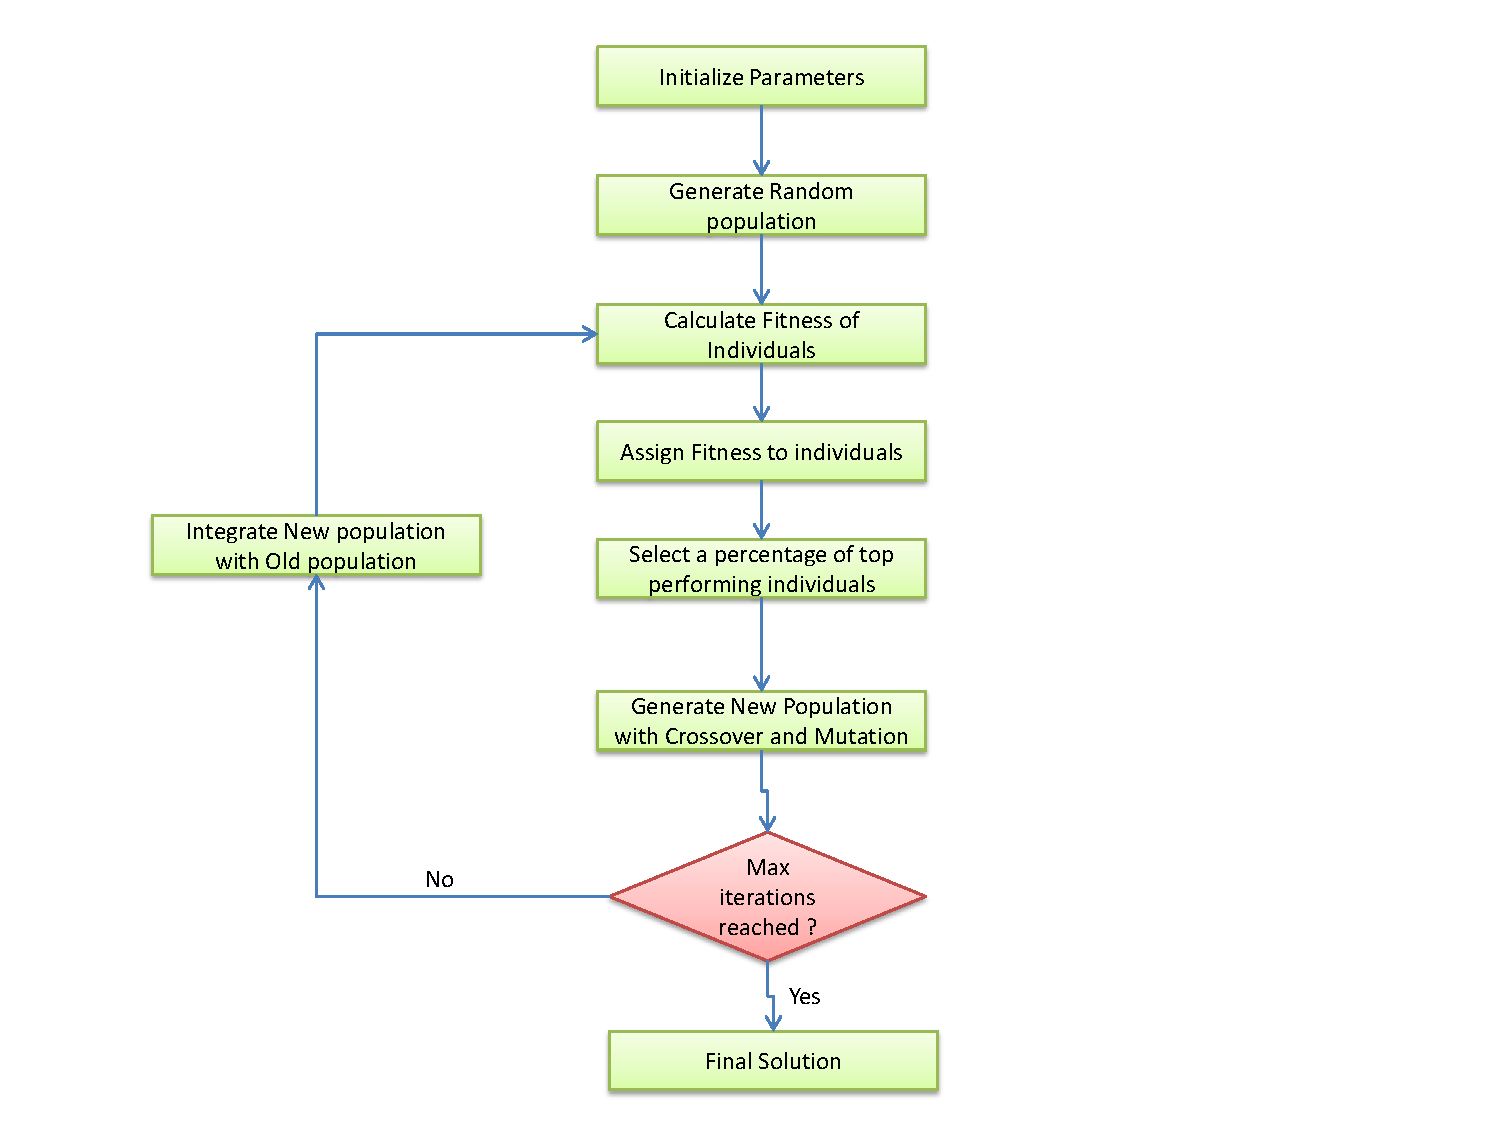
\includegraphics[width=5.0in,height=5.5in]{./pictures/GeneticAlgorithm.pdf}}
	\caption{Flow Chart for Genetic Algorithm}
	\label{fig:GeneticAlgorithmFlowChart}
	\end{center}
\end{figure}
\subsection{Introduction}
Genetic Algorithm (GA) is a stochastic search method that is based on the natural process of genetic evolution and the Darwinian concept of ``survival of the fittest'' \cite{DistributedHierarchicalGA,AcceleratingGA,AdaptiveSAGA,FamilyGA}. GA was initially developed for adaptive systems by Holland, but has then been widely used in the optimization field of study due to its effective exploration of the solution space as well as its relative success in multi-dimensional problems\cite{ParallelGASA,DistributedHierarchicalGA,FamilyGA}. 

The wide use of the GA algorithm can also be attributed to its generic algorithm structure as well as the ease of implementation of the algorithm \cite{FamilyGA,AdaptiveSAGA}. GA is application dependent and thus the designer needs to tailor the algorithm to his needs to obtain good results \cite{AcceleratingGA}.

The GA is generic since it defines no specific crossover, selector and mutation operator. It defines that these operators exist, but how exactly they perform their respective operations is up to the algorithm designer.

The GA search procedure involves searching the solution space through artificial evolution and natural selection\cite{FamilyGA,MultiPopGA,HybridIntelliGA}. An individual or point in the solution space is known as \emph{chromosome} in the literature \cite{HumanPassiveGA}. An initial set of chromosomes (referred to in the research as the \emph{population}), is randomly generated\cite{FamilyGA,HybridIntelliGA,AcceleratingGA,MultiPopGA}. 

Unlike other algorithms, GA does not concentrate on one point when searching the solution space, but concentrates on a wide range of points represented by the population \cite{DistributedHierarchicalGA,FamilyGA,HybridIntelliGA}\label{GASearchPoints}. Each chromosome in the solution space represents a string encoding of the problem parameters\cite{FamilyGA}. Encoding problem parameters also attributes to the wide use of the GA since difficult mathematical problems can now be easily modelled \cite{AcceleratingGA}.

The population is artificially evolved each iteration by using a set of stochastic operators\cite{SelfAdaptiveGA}. This set consists of a selection operator, crossover operator and mutation operator\cite{SelfAdaptiveGA,MultiPopGA}. Each operator plays an important role in emulating the evolutionary process. 

The selection operator is in charge of applying the \emph{objective function} to each chromosome in the population \cite{AdaptiveSAGA,HumanPassiveGA}. Depending on if the selection operator is setup for maximization of minimization, each individual is ranked based on its ``fitness'' or objective function value.

In figure \ref{fig:GeneticAlgorithmFlowChart} the selection operator is the first operation applied after a random starting population has been generated. It is also the first operation applied, when the algorithm starts a new generation.

In accordance with the Darwinian theory, only the fittest individuals are selected from the population \cite{HumanPassiveGA}. Based on the algorithm flow presented in figure \ref{fig:GeneticAlgorithmFlowChart}, the fittest individuals are only selected once the whole population has been assigned their respective fitness. 

The fittest individuals are copied and sent to the next phase of the algorithm, which is known as the \emph{Reproduction} phase \cite{HumanPassiveGA}. The reproduction phase can be observed in \ref{fig:GeneticAlgorithmFlowChart} as the operation where the new and old population are integrated.

Depending on how complicated the objective function is and how large the population is, the selection phase may be the most computationally expensive as well as time consuming \cite{AcceleratingGA}. The Reproduction phase mostly consists of string manipulations on the chromosome, to drive to search forward and it thus a phase which is completed quickly, especially if the string encoding is of a binary nature \cite{AcceleratingGA,AdaptiveSAGA}. These string manipulations occur through the application of the crossover and mutation operators \cite{ConstrainedGA}. 

The reproduction phase is where a new population is generated for the next generation to be evaluated by the selection operator. The reproduction is said to generate ``offspring'' from the selected fittest population who are in turn known as the ``parents'' of the offspring \cite{HumanPassiveGA,ConstrainedGA}. Reproduction will occur until a certain number of predefined generations are reached or a suitable solution is found to be greater/less than a certain fitness threshold that would indicate a good chromosome \cite{GATSP}.

There are two basic forms of the GA where both forms differ in the way that offspring and parents are handled \cite{FamilyGA}. The one form is called the \emph{generational} GA  and the other form is known as the \emph{steady-state} GA \cite{GeostatisticalGA,FamilyGA}.

With the generational GA the offspring are not immediately used in the next generation, instead they are kept in a pool until the pool reaches a certain size \cite{FamilyGA}. The offspring are then used to replace the parents entirely in the next generation \cite{FamilyGA}. In the steady-state GA the offspring are continually integrated with the population, thus offspring and parents occupy the same population pool every generation \cite{GeostatisticalGA,FamilyGA}.

The GA search process moves around in the search space using probabilistic rules rather than deterministic rules \cite{FamilyGA}. The probabilistic transition rules aid the algorithm to avoid local optima regions in the solution space \cite{HybridIntelliGA}. 

Some sequential search algorithms require that the objective function be differentiable \cite{ConstrainedGA}. These sequential algorithms use the derivative to obtain gradient information so that they can move in the solution space \cite{ConstrainedGA,SelfAdaptiveGA}. The derivative of the objective function may be used in to increase the efficiency of the GA, but is by no means a core requirement of the algorithm \cite{ConstrainedGA,HybridIntelliGA,SelfAdaptiveGA}. GA makes no assumptions about the solution space and primarily works on the information provided by the objective function \cite{ConstrainedGA,HybridIntelliGA}. 

In this section an overview of the Genetic Algorithm were presented. The core concept on which the algorithm is based upon was introduced and defined how the algorithm searches for solutions in a given domain. In the next section a general outline of the flow of the algorithm will be given.

\subsection{Flow of the algorithm}
Most of the core concepts of the genetic algorithm have been introduced in the previous section. To better understand the algorithm, a general overview of the algorithm will now be presented using algorithm~\ref{alg:GA} as reference point.

The GA algorithm is a population based algorithm and therefore needs to initialize its population. Each individual of the population represents a potential solution. Population initialization occurs on line 1 in algorithm~\ref{alg:GA}.

Before the algorithm can start \emph{evolving} its population, it first needs to determine each individual in the populations' fitness. The fitness of an individual is calculated using a fitness function $f(i)$.

Since the initial population has been evaluated, the algorithm is now in state to start its searching process, which starts at line 3 and ends at line 17.

The first part of the search process that is performed by the algorithm is to select a certain subset of the population. Typically this subset is the individuals of the population who have the highest fitness values. High fitness individuals are preferred as the fitness is an indication of good genes, which is to say, the solution the individual represents is of a high quality. This subset selection can be observed to occur on line 4.

All the individuals that are not in the subset are removed from the population. Once the subset selection has been completed, the algorithm is ready to enter the reproduction phase that ranges from line 6 -- 15.

The first step in the reproduction phase is where various individuals of the subset are mated together to produce a new offspring individual. Mating occurs through the use of the crossover operator. The purpose of the crossover operator is to take certain characteristics of the two mating individuals and combine them to form a new individual referred to as the offspring. Generation of new individuals with the crossover operator can be observed from line 7 -- 8

The second step of the reproduction phase is where mutation occurs. For each of the offspring generated by the crossover a mutation probability is calculated. If the calculated probability for a particular offspring is high enough, the algorithm enters the mutation phase. In the mutation phase, the offspring is mutated, which is to say, the solution represented by the individual is altered slightly to be different. Mutation can be seen to occur on line 9 -- 10.

Regardless whether offspring has been mutated or not, the resulting offspring is added to the new population. The reproduction phase continually loops, until the new population equals the size of the initial starting population. Once the new population has reached the sufficient size, the algorithm moves on to its next iteration.

The algorithm continually generates and evaluates new population until a predetermined stopping criterion has been met. Once the criterion has been met, the algorithm selects the individual with the highest fitness in the current population as its most optimal solution.

In section a general overview of genetic algorithm flow was presented. In the next section various characteristics that make up the genetic algorithm and have up and till now only been mentioned will be explained in much more detail.
\subsection{Important Genetic Algorithm characteristics}
In this section an overview on characteristics that make the GA search procedure unique will be presented. The first discussion will be on the initial population generation. Furthermore, for each operator namely, selection, mutation and elitism operators a brief overview will be given.

This section will conclude with a discussion on the efficiency of the GA algorithm.
\subsubsection{Initial Population Generation}
Initial population generation is the very first activity that the GA performs. Out of this population potential mating candidates are selected based on their fitness, which indicates the desirability. Generally the initial population is generated by means of randomization \cite{SelfAdaptiveGA}. Since the algorithm searches multiple points simultaneously in the solution space, it is desirable that the initial population have a wide diversity with regard to the solution they represent \cite{CombinedBranchBoundGA,DistributedHierarchicalGA}. By controlling the initial population generation we can control, to a small degree, the amount of exploration the algorithm does initially as well as avoid premature convergence \cite{CombinedBranchBoundGA}, therefore care must be taken in the selection of the particular randomization scheme that will be used to generate solutions.

In a survey done by Andrea Reese\cite{RandomNumberGA}, two randomization schemes are defined namely pseudo-random number generators (PRNGs) and quasi-random number generators (QRNGs). PRNGs where found to be heavily problem dependant, improving the search efficiency in some instances and in other instances having no considerable impact. QRNGs on the other hand, were shown to significantly improve the final solution produced by the GA as well as lowering the number of generations for the solution to be obtained \cite{RandomNumberGA}.

Not all GA algorithm use randomization entirely for their initial population generation. In research done by Amit Nagar, Sunderesh S. Heragu and Jorge Haddock\cite{CombinedBranchBoundGA} an algorithm is presented that generates an initial population through some aid of a branch-and-bound algorithm. The branch-and-bound algorithm provides the GA with an upper bound of acceptable solution in the solution space. The initial population is then randomly generated in the constrained space defined by the upper bound\cite{CombinedBranchBoundGA}.
\subsubsection{Selection Operator}
The Selection operator is the first operator to be applied to the population after each generation. This operator is in charge of evaluating the current population to determine which individuals will survive and which will be terminated \cite{CoactiveFuzzyGA,CombinedBranchBoundGA,ConstrainedGA}. The individuals who survive and thus have the highest fitness are moved to a ``mating pool'' \cite{HumanPassiveGA}. Individuals from this mating pool will be used in the reproduction phase to generate a new population \cite{AdaptiveSAGA,AcceleratingGA}.

By favouring high fitness individuals above low fitness individuals the operator guides the search towards better high quality solutions \cite{ConstrainedGA}. Care must be taken if the operator is too eager on high quality individuals since it may eliminate diversity in the population and thus result in premature convergence for certain problems \cite{ConstrainedGA}. If the solution space is known to have only one optimum, then a strict selection policy may be used, therefore directing the search into a gradient based direction \cite{ConstrainedGA}. In contrast, with a solution space that is known to have multiple optima, a forgiving selection policy might be more favourable since it allows the solution space to be more widely explored \cite{ConstrainedGA}.

The most widely adopted selection scheme is known as the \emph{Roulette Wheel} selection scheme \cite{ConstrainedGA,GeostatisticalGA,HybridBaldwinGA,CoactiveFuzzyGA}. With this scheme an individual is selected based on a probability defined by the fitness of the individual divided by the collective fitness of the population \cite{GeostatisticalGA}.
\subsubsection{Crossover Operator}
\label{sec:crossover}
The Crossover operator is usually the first operator applied to the population in the reproduction phase. The crossover operates exclusively on the chromosomes in the mating pool. This operator is the main process by which by the GA algorithm is able to diversify as well as exploit certain optimal regions \cite{CombinedBranchBoundGA,CoactiveFuzzyGA}. 

Crossover works by interchanging and matching two parent chromosomes randomly selected from the mating pool to produce a single chromosome known as the offspring \cite{FamilyGA,HumanPassiveGA,CoactiveFuzzyGA}. Since two chromosomes are combined or partially changed, some historical information is retained in the new chromosome \cite{FamilyGA}.

In some algorithms, like for instance, the one presented in Nagar et. al., before the crossover operator is applied to the two parent chromosomes, the parents are first evaluated to determine if they represent suboptimal regions\cite{CombinedBranchBoundGA}.

If either of the parents is from a suboptimal region, a disruption operator is applied that interchanges certain domain specific information between the parents. After the disruption operator is applied the crossover operator is applied \cite{CombinedBranchBoundGA}.

There are a variety of ways with which values are interchanged between chromosomes in the crossover operation i.e. Fixed point crossover, Two Point Crossover, Uniform Crossover and Gaussian Crossover. Fixed point crossover operates on binary parents where by a point is selected in one parent and then all other bits are replaced by the other parents bits \cite{HumanPassiveGA}. 

Two point crossover generates two random indices' which dictates a certain segment in the one parent to be interchanged with the other parent \cite{ConstrainedGA}. 

Uniform crossover is the most basic of all crossovers since it randomly selects bits from one parent to be replaced by another parents bits and is usually used when a large solution space must be search\cite{ParallelGASA,GeostatisticalGA}. 

Finally, the Gaussian crossover, interchanges bits between parents based on a Gaussian distribution \cite{ParallelGASA,GeostatisticalGA}. Depending on the state of the algorithm, crossover operators can also be interchanged or even paired if the algorithm needs better search performance for large or small solution spaces \cite{HetergeneousGA,ParallelGASA}.

Note, in all above crossovers it is assumed that the chromosomes are bit encoded, but these crossovers do require them to be. All these crossover operators are able to work on any encoding, it just depends on what is considered to be a ``bit'' if a non-binary encoding is used. 

\subsubsection{Mutation Operator}
The mutation operator is a probabilistic operator, which means it is applied infrequently and thus only with a certain probability will it be applied to parent solution. The operator typically changes some small in the solution regardless of the fitness of the chromosome \cite{HybridBaldwinGA,HumanPassiveGA}.

Given enough time, the mutation operator enables the algorithm to search the entire search space \cite{FamilyGA}. The operator also aids the algorithm with regard to escaping local optima in the solution space \cite{FamilyGA}.

Due to the way the crossover works, some information may be lost when it is replaced by other chromosomes bits \cite{AcceleratingGA,ConstrainedGA}. Mutation is a source of new information that is continuously inserted into the algorithm; hence it works against information loss \cite{CoactiveFuzzyGA,AcceleratingGA,ConstrainedGA}. 

Usually, the mutation operator has no previous information on the chromosome it is mutating, thus it is entirely possible that the mutation may modify the chromosome for the worse \cite{AcceleratingGA}. A worse solution might lead the algorithm out of local optima or lead it down a new path to find the global optima, but this isn't always the case and thus in the literature the probability of the mutation operator is set to be very low \cite{AdaptiveSAGA,FamilyGA,ConstrainedGA}.

In a survey done by Engelbrecht\cite{CompuIntelligenceIntro} another mutation operator is discussed. Instead of mutating a small part of randomly selected chromosomes, this operator generates new offspring to be inserted back into the population. The operator randomly generates a new chromosome and then using any of the previous discussed crossover operators (see page~\pageref{sec:crossover}).

The mutation operator isn't always simple random operations. In research done by Il-kwon Jeong and Ju-jang Lee, a mutation operator is presented that incorporates the Simulated Annealing algorithm. Th SA mutation operator generates a new chromosome whose fitness is also calculated. If the new chromosome fitness is worse than the chromosome to be mutated, then depending on the SA mutation temperature as well cooling schedule, the newly generated chromosome might replace the chromosome to be mutated, otherwise if the new chromosome has a better fitness than the chromosome to be mutated, it is replaced \cite{AdaptiveSAGA}.

\subsubsection{Elitism Operator}
The elitist operator differs from the crossover and mutation operator in a sense that, it doesn't modify the chromosomes in any way. Instead, the operator works on the population \cite{PatternDetectionGA}. The elitist operator ensures that the best chromosomes do not get lost from one population to the next, when the crossover and mutation operators are applied \cite{HetergeneousGA}. Thus the elitist operator is only applied after the crossover and mutation operators have generated a new population. 

The elitist selects a certain number of high quality chromosomes from the parent population and transfer them in the new population without any modification from the other two operators \cite{PatternDetectionGA}. 

The operator does not just move parents into the new population. The operator typically replaces sub par chromosomes in the new population with the higher quality parents \cite{RealParameterGASA}, therefore the elitist operator helps the algorithm retain knowledge gained from previous generations and prevents the best solution from extinction \cite{DynamicPenaltyGA}. 

Finally, the retainment of knowledge and best solution aids the algorithm with regard to global convergence \cite{SelfAdaptiveDataMiningGA}.

\subsubsection{Algorithm Efficiency}
The GA is a powerful, yet simple algorithm and tends to find good solutions given enough time, but the algorithm does have its disadvantages. One of the major disadvantages occurs when the GA is applied to problems that have very large solution spaces. In these problems, the population size is a very sensitive parameter\cite{AdaptiveGA,HetergeneousGA,SelfAdaptiveDataMiningGA,PatternDetectionGA}. If the population is too small the algorithm won't have enough diversity to search and tend to premature converge. 

A large population is preferred in large problem spaces, but then the algorithm is very computationally expensive since more time is spent evaluating than evolving new populations and the speed of the algorithm convergence decreases drastically. Hence, the population size must be fine tuned to achieve optimal performance in large problem spaces \cite{AdaptiveGA,CompuIntelligenceIntro}

Another disadvantage of GA is that it is memory intensive, most sequential algorithms search on a single point bases through the solution space. As discussed above (see page ~\pageref{GASearchPoints}), GA algorithms searches multiple points simultaneously and therefore requires more memory the keep track of all the possible solutions.

In conclusion, the algorithm has some sort of hill-climbing through the mutation operator, but the probability of the mutation operator is far too low for the algorithm to be considered to have a real hill-climbing capability.

\subsection{Genetic Algorithm on the FAP}
Continuing the trend of the SA and TS algorithms, the GA has also been applied to a wide variety of optimization problems and has on average obtained good results and in some cases better than all previous algorithms. Due to the success of the GA on other difficult problems, the GA algorithm has therefore also been applied to the FAP.

In the literature by Colombo and Allen\cite{ProblemDecompMIFAP} the authors developed a GA algorithm to be applied on the FAP. The authors also utilize the notion of dynamic programming, by decomposing the FAP problem into smaller sub problems. On average the solution quality is improved by using the technique but at the expensive of more complex and taxing evaluations that have to be performed\cite{ProblemDecompMIFAP}. 

The evaluations are more complex, since in most instances the sub problems (which are sub graphs) overlap with other sub problems, therefore more complex evaluations need to be performed taking into account the overlapping\cite{ProblemDecompMIFAP}. The authors report that the technique is viable to improve solution quality as long as the connectivity between the sub problem graphs is not too high \cite{ProblemDecompMIFAP}.

The results the authors obtained will now be represented.

\begin{table}
\centering
	\begin{tabular}{| c | c | c |}
	\hline
	Problem instance & GA & Cost 259 \\ \hline
	Siemens 1 & 2.60 & 2.20 \\ \hline
	Siemens 2 & 16.34 & 14.280 \\ \hline
	Siemens 3 & 6.37 & 5.19 \\ \hline
	Siemens 4 & 84.08 & 81.89 \\ \hline
	\end{tabular}
\caption{GA on Cost 259 Benchmark}
\end{table}

By critically evaluating the genetic algorithm if it would be applied to the FAP, the following disadvantages can be identified.

\paragraph{Diversity}
The GA algorithm continually operates on a set population that was randomly initialized in the beginning of the algorithm. The algorithm hence only has this set of generated genes in the initialized population to therefore evolve successive populations from.
If one disregard mutation, the GA algorithm is a process by which the optimal combinations of the starting genes are found. Thus, the GA algorithm purifies the starting population genes in an attempt to find those individual genes, which if combined into a single individual, will produce an optimal individual i.e. solution, therefore the genetic algorithm is very much reliant on the quality of the random generator used, hence the probability of the algorithm finding a particular desirable gene that is exhibited by the starting population is directly related to the rate of mutation, as mutation is the only means by which more diversity gets introduced in the GA algorithm.
\paragraph{Crossover}
The Crossover operation in the GA algorithm is the only means by which successive populations are generated and can therefore be regarded as the primary means by which the algorithm performs its search. As the crossover is defined in the standard algorithm, certain parts of both parents are copied and combined to form a new individual. With regard to the FAP, if each individual represents a frequency plan, the crossover operation would copy certain cells from the two parent plans. This is not desirable, since a single channel within a cell can generate large interference that overshadows the rest of the channels that generate low interference in the cell. Thus, for the GA to generate high quality solutions on the FAP, the algorithm would be better off utilizing a crossover operation which works on individual channels assigned rather than cells. Crossover operation is also a memory and computational expensive operation since individuals need to be constantly created and values need to be copied to these new individuals from the respective parents.
\paragraph{Mutation}
Mutation is the primary means by which more diversity is introduced in the GA population. Typically the mutation value is set to a low probability due to mutation actually \emph{modifying} individuals and not introducing \emph{new} individuals, therefore there is a possibility that a mutation might alter an excellent solution in such a way, that the solution is suddenly one of the worst solutions. With regard to the FAP, the low probability of mutation is not desirable, as the FAP search space is huge and therefore requires constant diversity to be introduced to accurately explore the FAP search space. A possible good mutation would be one that is slightly more intelligent than the standard mutation operator, which just randomly modifies a selected individual. An intelligent mutation, would be one that takes into account the recent history of the individual as well as the history of the population and based on the collective gathered knowledge alter or \emph{mutate} a particular individual.
\section {Summary}
In this chapter a presentation was given of meta-heuristic algorithms. A definition was given on what it means for an algorithm to be classified as being of a meta-heuristic nature and also what characteristic these algorithms must exhibit.

Three meta-heuristic algorithms were discussed in this chapter. For each algorithm a flow chart was presented which visually depicts the general flow of the algorithm along with a discussion on how the algorithm works as well as the various characteristics that make the algorithm unique.

For each algorithm, a brief overview of literature using the particular algorithm was given as well as a series of brief discussions on some of the disadvantages or challenges that will be faced when applying the particular algorithm on the FAP.

The first algorithm discussed was the Tabu search algorithm and the second algorithm was the simulated annealing algorithm. The chapter concluded with a discussion on the Genetic algorithm. In the next chapter a discussion will be given on a class of algorithm that is relatively new to optimization research, namely the Swarm Intelligence class of algorithms.

In the table below, the algorithms discussed in this chapter and their performance on the Cost 259 set of benchmarks have been summarised.\\
\begin{table}[h]
\label{tbl:summaryMetaTable}
\begin{center}
	\begin{tabular}{| c | c | c | c | c |}
	\hline
	Problem instance & TS & SA & GA & Cost 259 \\ \hline
	Siemens 1 & 2.7692 & 23.00 & 2.60 & 2.20 \\ \hline
	Siemens 2 & 14.9360 & 14.75 & 16.34 & 14.280 \\ \hline
	Siemens 3 & 6.6496 & 52.55 & 6.37 & 5.19 \\ \hline
	Siemens 4 & 110.9725 & 80.80 & 84.08 & 81.89 \\ \hline
	\end{tabular}
\caption{Summary of algorithm performance on the Cost 259 benchmark}
\end{center}
\end{table}

For each algorithm presented in this chapter a critical evalaution was presented if the algorithm were to be applied on the FAP. These evaluations are based on the observations and considerations on theoretical implementations of these algorithms by the author of this dissertation.
